\documentclass[a4paper, 12pt]{article}
\usepackage[utf8]{inputenc}
\usepackage[english, ukrainian]{babel}

\usepackage{amsmath, amssymb}
\usepackage{multicol}
\usepackage{graphicx}
\usepackage{float}

\allowdisplaybreaks
\setlength\parindent{0pt}
\numberwithin{equation}{subsection}

\usepackage{hyperref}
\hypersetup{unicode=true,colorlinks=true,linktoc=all,linkcolor=red}

\numberwithin{equation}{subsection}

\renewcommand{\bf}[1]{\textbf{#1}}
\renewcommand{\it}[1]{\textit{#1}}
\newcommand{\bb}[1]{\mathbb{#1}}
\renewcommand{\cal}[1]{\mathcal{#1}}

\renewcommand{\epsilon}{\varepsilon}
\renewcommand{\phi}{\varphi}

\DeclareMathOperator{\diam}{diam}
\DeclareMathOperator{\rang}{rang}
\DeclareMathOperator{\const}{const}

\newenvironment{system}{%
  \begin{equation}%
    \left\{%
      \begin{aligned}%
}{%
      \end{aligned}%
    \right.%
  \end{equation}%
}
\newenvironment{system*}{%
  \begin{equation*}%
    \left\{%
      \begin{aligned}%
}{%
      \end{aligned}%
    \right.%
  \end{equation*}%
}

\makeatletter
\newcommand*{\relrelbarsep}{.386ex}
\newcommand*{\relrelbar}{%
  \mathrel{%
    \mathpalette\@relrelbar\relrelbarsep%
  }%
}
\newcommand*{\@relrelbar}[2]{%
  \raise#2\hbox to 0pt{$\m@th#1\relbar$\hss}%
  \lower#2\hbox{$\m@th#1\relbar$}%
}
\providecommand*{\rightrightarrowsfill@}{%
  \arrowfill@\relrelbar\relrelbar\rightrightarrows%
}
\providecommand*{\leftleftarrowsfill@}{%
  \arrowfill@\leftleftarrows\relrelbar\relrelbar%
}
\providecommand*{\xrightrightarrows}[2][]{%
  \ext@arrow 0359\rightrightarrowsfill@{#1}{#2}%
}
\providecommand*{\xleftleftarrows}[2][]{%
  \ext@arrow 3095\leftleftarrowsfill@{#1}{#2}%
}
\makeatother

\newcommand{\NN}{\mathbb{N}}
\newcommand{\ZZ}{\mathbb{Z}}
\newcommand{\QQ}{\mathbb{Q}}
\newcommand{\RR}{\mathbb{R}}
\newcommand{\CC}{\mathbb{C}}

\newcommand{\Max}{\displaystyle\max\limits}
\newcommand{\Sup}{\displaystyle\sup\limits}
\newcommand{\Sum}{\displaystyle\sum\limits}
\newcommand{\Int}{\displaystyle\int\limits}
\newcommand{\Iint}{\displaystyle\iint\limits}
\newcommand{\Lim}{\displaystyle\lim\limits}

\newcommand*\diff{\mathop{}\!\mathrm{d}}

\newcommand*\rfrac[2]{{}^{#1}\!/_{\!#2}}


\title{{\Huge МАТЕМАТИЧНА ФІЗИКА}}
\author{Скибицький Нікіта}
\date{\today}

\usepackage{amsthm}
\usepackage[dvipsnames]{xcolor}
\usepackage{thmtools}
\usepackage[framemethod=TikZ]{mdframed}

\theoremstyle{definition}
\mdfdefinestyle{mdbluebox}{%
	roundcorner = 10pt,
	linewidth=1pt,
	skipabove=12pt,
	innerbottommargin=9pt,
	skipbelow=2pt,
	nobreak=true,
	linecolor=blue,
	backgroundcolor=TealBlue!5,
}
\declaretheoremstyle[
	headfont=\sffamily\bfseries\color{MidnightBlue},
	mdframed={style=mdbluebox},
	headpunct={\\[3pt]},
	postheadspace={0pt}
]{thmbluebox}

\mdfdefinestyle{mdredbox}{%
	linewidth=0.5pt,
	skipabove=12pt,
	frametitleaboveskip=5pt,
	frametitlebelowskip=0pt,
	skipbelow=2pt,
	frametitlefont=\bfseries,
	innertopmargin=4pt,
	innerbottommargin=8pt,
	nobreak=true,
	linecolor=RawSienna,
	backgroundcolor=Salmon!5,
}
\declaretheoremstyle[
	headfont=\bfseries\color{RawSienna},
	mdframed={style=mdredbox},
	headpunct={\\[3pt]},
	postheadspace={0pt},
]{thmredbox}

\declaretheorem[style=thmbluebox,name=Теорема,numberwithin=subsubsection]{theorem}
\declaretheorem[style=thmbluebox,name=Лема,numberwithin=subsubsection]{lemma}
\declaretheorem[style=thmbluebox,name=Твердження,numberwithin=subsubsection]{proposition}
\declaretheorem[style=thmbluebox,name=Принцип,numberwithin=subsubsection]{th_principle}
\declaretheorem[style=thmbluebox,name=Закон,numberwithin=subsubsection]{law}
\declaretheorem[style=thmbluebox,name=Закон,numbered=no]{law*}
\declaretheorem[style=thmbluebox,name=Формула,numberwithin=subsubsection]{th_formula}
\declaretheorem[style=thmbluebox,name=Рівняння,numberwithin=subsubsection]{th_equation}
\declaretheorem[style=thmbluebox,name=Умова,numberwithin=subsubsection]{th_condition}
\declaretheorem[style=thmbluebox,name=Наслідок,numberwithin=subsubsection]{corollary}

\declaretheorem[style=thmredbox,name=Приклад,numberwithin=subsubsection]{example}
\declaretheorem[style=thmredbox,name=Приклади,sibling=example]{examples}

\declaretheorem[style=thmredbox,name=Властивість,numberwithin=subsubsection]{property}
\declaretheorem[style=thmredbox,name=Властивості,sibling=property]{properties}

\mdfdefinestyle{mdgreenbox}{%
	skipabove=8pt,
	linewidth=2pt,
	rightline=false,
	leftline=true,
	topline=false,
	bottomline=false,
	linecolor=ForestGreen,
	backgroundcolor=ForestGreen!5,
}
\declaretheoremstyle[
	headfont=\bfseries\sffamily\color{ForestGreen!70!black},
	bodyfont=\normalfont,
	spaceabove=2pt,
	spacebelow=1pt,
	mdframed={style=mdgreenbox},
	headpunct={ --- },
]{thmgreenbox}

\mdfdefinestyle{mdblackbox}{%
	skipabove=8pt,
	linewidth=3pt,
	rightline=false,
	leftline=true,
	topline=false,
	bottomline=false,
	linecolor=black,
	backgroundcolor=RedViolet!5!gray!5,
}
\declaretheoremstyle[
	headfont=\bfseries,
	bodyfont=\normalfont\small,
	spaceabove=0pt,
	spacebelow=0pt,
	mdframed={style=mdblackbox}
]{thmblackbox}

\declaretheorem[name=Вправа,numberwithin=subsubsection,style=thmblackbox]{exercise}
\declaretheorem[name=Зауваження,numberwithin=subsubsection,style=thmgreenbox]{remark}
\declaretheorem[name=Визначення,numberwithin=subsubsection,style=thmblackbox]{definition}

\newtheorem{problem}{Задача}[subsection]
\newtheorem{sproblem}[problem]{Задача}
\newtheorem{dproblem}[problem]{Задача}
\renewcommand{\thesproblem}{\theproblem$^{\star}$}
\renewcommand{\thedproblem}{\theproblem$^{\dagger}$}
\newcommand{\listhack}{$\empty$\vspace{-2em}} 

\theoremstyle{remark}
\newtheorem*{solution}{Розв'язок}


\begin{document}

\tableofcontents

\setcounter{section}{4}
\setcounter{subsection}{6}
\setcounter{subsubsection}{0}
\setcounter{equation}{11}

\subsubsection{Задача на власні значення для оператора Лапласа}

Причини порушення єдиності розв'язку у внутрішньої граничної задачі \seqref{4.6.9} і зовнішньої граничної задачі \seqref{4.6.10} різні. \medskip

Для того щоб зрозуміти причину існування нетривіального розв'язку у задачі \seqref{4.6.9} розглянемо більш загальну однорідну задачу з параметром:
\begin{system}
	\label{eq:4.6.12}
	& \Delta u(x) + \lambda u(x) = 0, \quad x \in \Omega, \\
	& \left. \ell_i u \right|_S = 0
\end{system}

Розв'язком цієї задачі будемо вважати таку множину значень параметру $\lambda$, при яких існує нетривіальний розв'язок граничної задачі \eqref{eq:4.6.12}, і самі розв'язки, що відповідають цим значенням параметру $\lambda$, які називають власними функціями. Неважко зрозуміти, що \eqref{eq:4.6.12} є узагальнення задачі Штурма--Ліувілля для оператора Лапласа. \medskip

Застосовуючи функцію Гріна $G_i(x, y)$ для оператора Лапласа граничної задачі, яка відповідає типу граничної умови, можемо звести \eqref{eq:4.6.12} до однорідного інтегрального рівняння Фредгольма другого роду з ермітовим полярним ядром:
\begin{equation}
	\label{eq:4.6.13}
	u(x) = \lambda \Iiint_\Omega G_i(x, y) u(y) \diff y.
\end{equation}

Оскільки множина характеристичних чисел ермітового ядра не порожня, то існує дійсне значення параметру $\lambda = \lambda_0$, такі що рівняння \eqref{eq:4.6.13} при цьому значені має нетривіальний розв'язок $u(x) = u_0(x)$. Тобто $\lambda_0, u_0(x)$ --- характеристичне число і власна функція рівняння \eqref{eq:4.6.13}, а значить і еквівалентної граничної задачі \eqref{eq:4.6.12}. \medskip

Таким чином, якщо для граничної задачі
\begin{system}
	\label{eq:4.6.14}
	& \Delta u(x) + k^2 u(x) = -F(x), \quad x \in \Omega, \\
	& \left. \ell_i u(x) \right|_{x \in S} = 0
\end{system}
реалізується ситуація, що число $ k^2$  співпадає з одним з характеристичних чисел оператора Лапласа для області   з заданим типом граничних умов, то розв'язок задачі \eqref{eq:4.6.14} для довільного вільного члена рівняння взагалі кажучи не існує. \medskip

Зрозуміло, що \eqref{eq:4.6.14} через функцію Гріна  можна звести до інтегрального рівняння
\begin{equation}
	\label{eq:4.6.15}
	u(x) = k^2 \Iiint_\Omega G_i(x, y) u(y) \diff y + F_1(x),
\end{equation}
де $F_1(x) = \Iiint_\Omega G_i(x, y) F(y) \diff y$. \medskip

Третя теорема Фредгольма для інтегральних рівнянь стверджує, що інтегральне рівняння \eqref{eq:4.6.15}, у випадку коли $k^2$ --- характеристичне число має розв'язок тоді і лише тоді, коли вільний член $F_1$ ортогональний усім розв'язкам однорідного рівняння \eqref{eq:4.6.13} при $\lambda = k^2$ а сам розв'язок неєдиний і визначається з точністю до лінійної оболонки натягнутої на систему власних функцій, що відповідають заданому значенню характеристичного числа. \medskip

Розглянемо тепер природу неєдиності розв'язку зовнішньої задачі \seqref{4.6.10}. Треба відмітити, що для зовнішніх задач рівняння Лапласа умова регулярності забезпечувала єдиність розв'язку. Для граничної задачі рівняння Гельмгольца в тривимірному просторі вимога лише затухання розв'язку на нескінченості вже не дає можливість виділити єдиний розв'язок. \medskip

При розв'язанні зовнішніх задач для рівняння Гельмгольца як правило цікавими є дві основні задачі:
\begin{itemize}
	\item Розповсюдження хвилі від тіла в нескінченість, коли тіло є джерелом виникнення періодичних коливань.
	\item Розповсюдження хвилі з нескінченості і взаємодія її з тілом, в цьому випадку відбувається дифракція.
\end{itemize}

Нагадаємо, що для тривимірного простору у рівняння Гельмгольца є фундаментальні розв'язки 
\begin{equation}
	\label{eq:4.6.16}
	q_k^\pm(x) = \frac{e^{\pm i k |x|}}{4 \pi |x|}
\end{equation}
які є комплексними амплітудами періодичних сферичних хвиль
\begin{equation}
	\label{eq:4.6.17}
	u_\pm(r, t) = \frac{\exp\left\{i \omega \left( t \pm \frac{r}{a} \right)\right\}}{4 \pi r}
\end{equation}
та, при цьому згадаємо, що $k = \omega  a$, $r = |x|$. \medskip

Легко перевірити, що сферичні хвилі $u_\pm(r, t)$ є розв'язками однорідного хвильового рівняння в тривимірному випадку. \medskip

Аналізуючи нахил прямих $t \pm r / a = \const$, можна зрозуміти, що $u_-(r, t)$ відповідає сферичній хвилі, яка прямує на нескінченість зі швидкістю $a$, а $u_+(r, t)$ відповідає хвилі як прямує з нескінченості зі швидкістю $-a$. \medskip

\begin{definition}
	Для виділення єдиного розв'язку зовнішньої задачі задаються умови поведінки розв'язку задачі в нескінченно віддаленій точці. Ці умови називають \textit{умовами випромінювання} або \textit{умовами Зомерфельда}:
	\begin{gather}
		\label{eq:4.6.18}
		u(x) = O(1/|x|), \qquad \frac{\partial u(x)}{\partial |x|} - i k u(x) = o(1/|x|), \quad |x| \to \infty, \\
		\label{eq:4.6.19}
		u(x) = O(1/|x|), \qquad \frac{\partial u(x)}{\partial |x|} + i k u(x) = o(1/|x|), \quad |x| \to \infty.
	\end{gather}
\end{definition}

Умова \eqref{eq:4.6.18} відповідає хвилям, що уходять на нескінченість, \eqref{eq:4.6.19} – хвилям, що приходять з нескінченості. \medskip

Саме умови \eqref{eq:4.6.18} і \eqref{eq:4.6.19} забезпечують єдність розв'язку зовнішніх граничних задач для рівняння Гельмгольца. \medskip

Для доведення цього факту можна скористатися формулами інтегрального представлення розв'язку однорідного рівняння Гельмгольца ($\Delta u + k^2 u = 0$):
\begin{equation}
	\label{eq:4.6.20}
	u(x) = -\Iint_S \left( \frac{e^{\pm i k |x - y|}}{4 \pi |x - y|} \frac{\partial u(y)}{\partial \vec n} - u(y) \frac{\partial}{\partial \vec n_y} \frac{e^{\pm i k |x - y|}}{4 \pi |x - y|} \right) \diff S_y.
\end{equation}

Формула \eqref{eq:4.6.20} є аналогом формули \seqref{4.5.6} отриманої для представлення розв'язків рівняння Лапласа. \medskip

Записавши \eqref{eq:4.6.20} для сфери $S_R(0)$ і спрямовуючи її радіус до нескінченості, а також враховуючи умови Зомерфельда \eqref{eq:4.6.18} для знака плюс та \eqref{eq:4.6.19} для знаку мінус ми отримаємо, що $u(x) \equiv 0$. \medskip

У випадку рівняння Гельмгольца на площині умови Зомерфельда мають вигляд:
\begin{gather}
	\label{eq:4.6.21}
	u(x) = O\left(1/\sqrt{|x|}\right), \qquad \frac{\partial u(x)}{\partial |x|} - i k u(x) = o\left(1/\sqrt{|x|}\right), \quad |x| \to \infty, \\
	\label{eq:4.6.22}
	u(x) = O\left(1/\sqrt{|x|}\right), \qquad \frac{\partial u(x)}{\partial |x|} + i k u(x) = o\left(1/\sqrt{|x|}\right), \quad |x| \to \infty.
\end{gather}

\subsection{Функції Бесселя та їх властивості}

При знаходженні розв'язків рівняння Пуассона та Гельмгольца в областях циліндричної форми, рівняння теплопровідності та хвильового рівняння в кругових та циліндричних областях з'являється необхідність записати розв'язки наступних звичайних диференціальних рівняння другого порядку з степеневими коефіцієнтами:
\begin{gather}
	\label{eq:4.7.1}
	x^2 y'' + x y' + (x^2 - \nu^2) y = 0, \\
	\label{eq:4.7.2}
	x^2 y'' + x y' - (x^2 + \nu^2) y = 0.
\end{gather}

В рівняннях \eqref{eq:4.7.1}, \eqref{eq:4.7.2} $\nu$ є числовий параметр.

\begin{definition}
	Рівняння \eqref{eq:4.7.1} називають рівнянням Бесселя порядку $\nu$, а рівняння \eqref{eq:4.7.2} називають рівнянням Бесселя уявного аргументу порядку $\nu$.
\end{definition}

Легко показати, що рівняння \eqref{eq:4.7.2} можна отримати з рівняння \eqref{eq:4.7.1} якщо в \eqref{eq:4.7.1} ввести заміну незалежної змінної $\xi = i x$, цей факт і пояснює назву рівняння \eqref{eq:4.7.2}. \medskip

Знайти розв'язок цих рівнянь у вигляді елементарних функцій не вдається, тому враховуючи поліноміальний вигляд коефіцієнтів рівняння, можна побудувати розв'язок рівнянь у вигляді узагальненого степеневого ряду.
\begin{equation}
	\label{eq:4.7.3}
	y(x) = x^\rho (a_0 + a_1 x + a_2 x^2 + \ldots),
\end{equation}
де $\rho, a_0, a_1, \ldots$ --- невідомі коефіцієнти. \medskip

Підставимо \eqref{eq:4.7.3} у \eqref{eq:4.7.1} і зберемо коефіцієнти при однакових степенях змінної $x$:
\begin{equation}
	\label{eq:4.7.4}
	(\rho^2 - \nu^2) a_0 x^\rho + ((\rho + 1)^2 - \nu^2) a_1 x^{\rho + 1} + \Sum_{k = 2}^\infty \left( ((\rho + k)^2 - \nu^2) a_k + a_{k - 2} \right) x^{\rho + k} = 0.
\end{equation}

З \seqref{4.6.4} отримаємо рівності для визначення коефіцієнтів.
\begin{equation}
	\label{eq:4.7.5}
	\begin{aligned}
		\rho^2 - \nu^2 &= 0, \\
		a_1 &= 0, \\
		((\rho + k)^2 - \nu^2) a_k + a_{k - 2} &= 0.
	\end{aligned}
\end{equation}

З першого рівняння \eqref{eq:4.7.5} маємо:
\begin{equation}
	\label{eq:4.7.6}
	\rho = \nu, \quad \rho = - \nu.
\end{equation}

Оберемо перше значення, а саме $\rho = \nu$, тоді отримаємо
\begin{equation}
	\label{eq:4.7.7}
	a_k = - \frac{a_{k - 2}}{k (2 \nu + k)}, \quad k = 2, 3, \ldots
\end{equation}

Враховуючи \eqref{eq:4.7.7} та друге співвідношення \eqref{eq:4.7.5} маємо $a_1 = a_3 = \ldots = a_{2k + 1} = \ldots = 0$. \medskip

Для коефіцієнтів з парними індексами з формули \eqref{eq:4.7.7} легко отримати 
\begin{equation}
	\label{eq:4.7.8}
	a_{2k} = (-1)^k \cdot \frac{a_0}{2^{2k} \cdot (\nu + 1) \cdot (\nu + 2) \cdot \ldots \cdot (\nu + k) \cdot k!}
\end{equation}

Обираючи
\begin{equation}
	\label{eq:4.7.9}
	a_0 = \frac{1}{2^\nu \Gamma(\nu + 1)}
\end{equation}
і підставляючи значення коефіцієнтів в \eqref{eq:4.7.3} отримаємо 
\begin{equation}
	\label{eq:4.7.10}
	J_\nu(x) = \Sum_{k = 0}^\infty \frac{(-1)^k}{\Gamma(k + \nu + 1) k!} \left(\frac{x}{2}\right)^{2k + \nu}.
\end{equation}

Обираючи друге значення параметру $\rho = - \nu$, отримаємо 
\begin{equation}
	\label{eq:4.7.10'}
	J_{-\nu}(x) = \Sum_{k = 0}^\infty \frac{(-1)^k}{\Gamma(k - \nu + 1) k!} \left(\frac{x}{2}\right)^{2k - \nu}.
\end{equation}

Відмітимо, що визначення функції $J_{-\nu}(x)$ є коректним лише для не цілих значень параметру $\nu$, оскільки визначення $a_0$ за формулою \eqref{eq:4.7.9} при $\nu = - n$ не має змісту, оскільки $\Gamma(0) = \Gamma(-1) = \ldots = \Gamma(-n) = \infty$. \medskip

Змінюючи в формулі \eqref{eq:4.7.10'} індекс сумування $k = k' + n$, отримаємо
\begin{equation}
	\label{eq:4.7.11}
	J_{-n}(x) = (-1)^n \Sum_{k'=1}^\infty \frac{(-1)^{k'}}{\Gamma(k'+n+1)\Gamma(k'+1)} \left(\frac{x}{2}\right)^{2k'+n}=(-1)^n J_n(x).
\end{equation}

Остання рівність свідчить про лінійну залежність функцій $J_n(x)$ та $J_{-n}(x)$ і таким чином лінійна комбінація цих функцій не може складати загальний розв'язок рівняння Бесселя. \medskip

Другий лінійно незалежний розв'язок рівняння Бесселя для довільного значення параметру $\nu$, взагалі кажучи не представляється у вигляді узагальненого степеневого ряду \eqref{eq:4.7.3}, утворимо спеціальну лінійну комбінацію для нецілих значень параметру $\nu$:
\begin{equation}
	\label{eq:4.7.12}
	N_\nu(x) = \frac{\cos (\nu \pi) J_\nu(x) - J_{-\nu}(x)}{\sin(\nu\pi)}, \quad \nu \ne n.
\end{equation}

Для $\nu = n$, враховуючи попередні викладки, маємо що чисельник і знаменник тотожно перетворюються в нуль, тобто маємо невизначеність типу $0/0$. Розкриємо невизначеність за допомогою правила Лопіталя:
\begin{equation}
	\label{eq:4.7.12'}
	N_n(x) = \frac{1}{\pi} \left( \left( \frac{\partial J_\nu(x)}{\partial \nu} \right)_{\nu = n} - (-1)^n \left( \frac{\partial J_{-\nu}(x)}{\partial \nu} \right)_{\nu = n} \right)
\end{equation}

Покажемо, що функція $N_n(x)$ задовольняє рівняння \eqref{eq:4.7.1}. Дійсно, позначимо диференціальний оператор 
\begin{align}
	\label{eq:4.7.13}
	L(J_\nu) &= J_\nu'' + \frac{1}{x} \cdot J_\nu' + \left( 1 - \frac{\nu^2}{x^2} \right) \cdot J_\nu = 0, \\
	\label{eq:4.7.13'}
	L(J_{-\nu}) &= J_{-\nu}'' + \frac{1}{x} \cdot J_{-\nu}' + \left( 1 - \frac{\nu^2}{x^2} \right) \cdot J_{-\nu} = 0.
\end{align}

Продиференціюємо останні рівності по $\nu$, та отримаємо:
\begin{equation}
	L \left( \frac{\partial J_\nu}{\partial \nu} \right) - \frac{2 \nu}{x^2} \cdot J_\nu = 0, \qquad L \left( \frac{\partial J_{-\nu}}{\partial \nu} \right) - \frac{2 \nu}{x^2} \cdot J_{-\nu} = 0.
\end{equation}

Помножимо перше рівняння на $(+1)^n$, друге рівняння на $(-1)^n$, віднімемо від першого рівняння друге, отримаємо:
\begin{equation}
	L \left( \frac{\partial J_\nu}{\partial \nu} \right) - (-1))^n L \left( \frac{\partial J_{-\nu}}{\partial \nu} \right) - \frac{2 \nu}{x^2} (J_\nu - (-1)^n J_{-\nu}) = 0.
\end{equation}

Остаточний вигляд функції Бесселя другого роду
\begin{equation}
	\begin{aligned}
		N_n(x) &= -\frac{1}{\pi} \Sum_{k = 0}^{n - 1} \frac{(n - k - 1)!}{k!} \left(\frac{x}{2}\right)^{2 k - n} + \frac{2}{\pi} \cdot J_n(x) \cdot \ln \frac{x}{2} - \\
		& \quad - \frac{1}{\pi} \Sum_{k = 0}^\infty \frac{(-1)^k (x / 2)^{2 k + n}}{k! (k + n)!} \left( \Psi(k + n + 1) + \Psi(k + 1) \right).
	\end{aligned}
\end{equation}

\begin{remark}
	Дуже часто функцію Бесселя другого роду $N_\nu(x)$ називають \textit{функцією Вебера}.
\end{remark}

Важливою властивістю функцій Бесселя є асимптотичний характер поведінки цих функцій на нескінченості. Вводячи функцію $y(x) = V(x) / \sqrt{x}$, підставляючи її в рівняння Бесселя отримаємо рівняння  
\begin{equation}
	V'' + \left( 1 - \frac{\nu^2 - 0.25}{x^2} \right) V = 0.
\end{equation}

Розв'язки останнього рівняння можна представити для $x \to \infty $ у вигляді 
\begin{equation}
	V(x) = \gamma \cdot \sin(x + \delta) + O\left(\frac{1}{x}\right),
\end{equation}
і, відповідно,
\begin{equation}
	y(x) = \gamma \cdot \frac{\sin(x + \delta)}{\sqrt{x}} + O\left(\frac{1}{x^{3/2}}\right).
\end{equation}

Додаткові дослідження дозволяють отримати, наступні асимптотичні формули при $x \to \infty$:
\begin{align}
	\label{eq:4.7.14}
	J_\nu(x) &= \sqrt{\frac{2}{\pi x}} \cdot \cos \left( x - \frac{\nu \pi}{2} - \frac{\pi}{4} \right) + O\left(\frac{1}{x^{3/2}}\right), \\
	\label{eq:4.7.14'}
	N_\nu(x) &= \sqrt{\frac{2}{\pi x}} \cdot \sin \left( x - \frac{\nu \pi}{2} - \frac{\pi}{4} \right) + O\left(\frac{1}{x^{3/2}}\right).
\end{align}

Останні формули свідчать про те, що функції Бесселя як першого так і другого роду мають злічену кількість нулів, тобто рівняння $J_\nu(x) = 0$, $N_\nu(x) = 0$  мають злічену кількість коренів, які для великих значень аргументу $x$ асимптотично прямують до нулів тригонометричних функцій $\cos \left( x - \frac{\nu \pi}{2} - \frac{\pi}{4} \right)$, $\sin \left( x - \frac{\nu \pi}{2} - \frac{\pi}{4} \right)$. А самі функції Бесселя ведуть себе як $O(1/\sqrt{x})$, $x \to \infty$. \medskip

Аналіз формул \eqref{eq:4.7.10} та \eqref{eq:4.7.14} показує, що при $x \to 0$:
\begin{gather}
	J_n(x) \approx \frac{1}{n!} \left( \frac{x}{2} \right)^n, \quad n = 0, 1, 2, \ldots, \\
	N_n(x) \approx - \frac{(n - 1)!}{\pi} \left( \frac{x}{2} \right)^n \to \infty, \\
	N_0(x) = \frac{2}{\pi} \ln \frac{x}{2} \to \infty.
\end{gather}

Важливою властивістю функцій Бесселя першого та другого роду є рекурентні формули, яким задовольняють функції Бесселя: 
\begin{gather}
	\label{eq:4.7.15}
	\frac{\diff}{\diff x} J_\nu(x) + \frac{\nu}{x} J_\nu(x) = J_{\nu - 1}(x), \qquad \frac{\diff}{\diff x} J_\nu(x) - \frac{\nu}{x} J_\nu(x) = - J_{\nu + 1}(x), \\
	\label{eq:4.7.16}
	\frac{\diff}{\diff x} N_\nu(x) + \frac{\nu}{x} N_\nu(x) = N_{\nu - 1}(x), \qquad \frac{\diff}{\diff x} N_\nu(x) - \frac{\nu}{x} N_\nu(x) = - N_{\nu + 1}(x).
\end{gather}

Виключаючи з двох співвідношень похідну, можна зв'язати між собою функції Бесселя трьох сусідніх порядків. \medskip

Для прикладу наведемо графіки функцій Бесселя $J_3(x)$ та $N_3(x)$:
\begin{figure}[H]
	\centering
	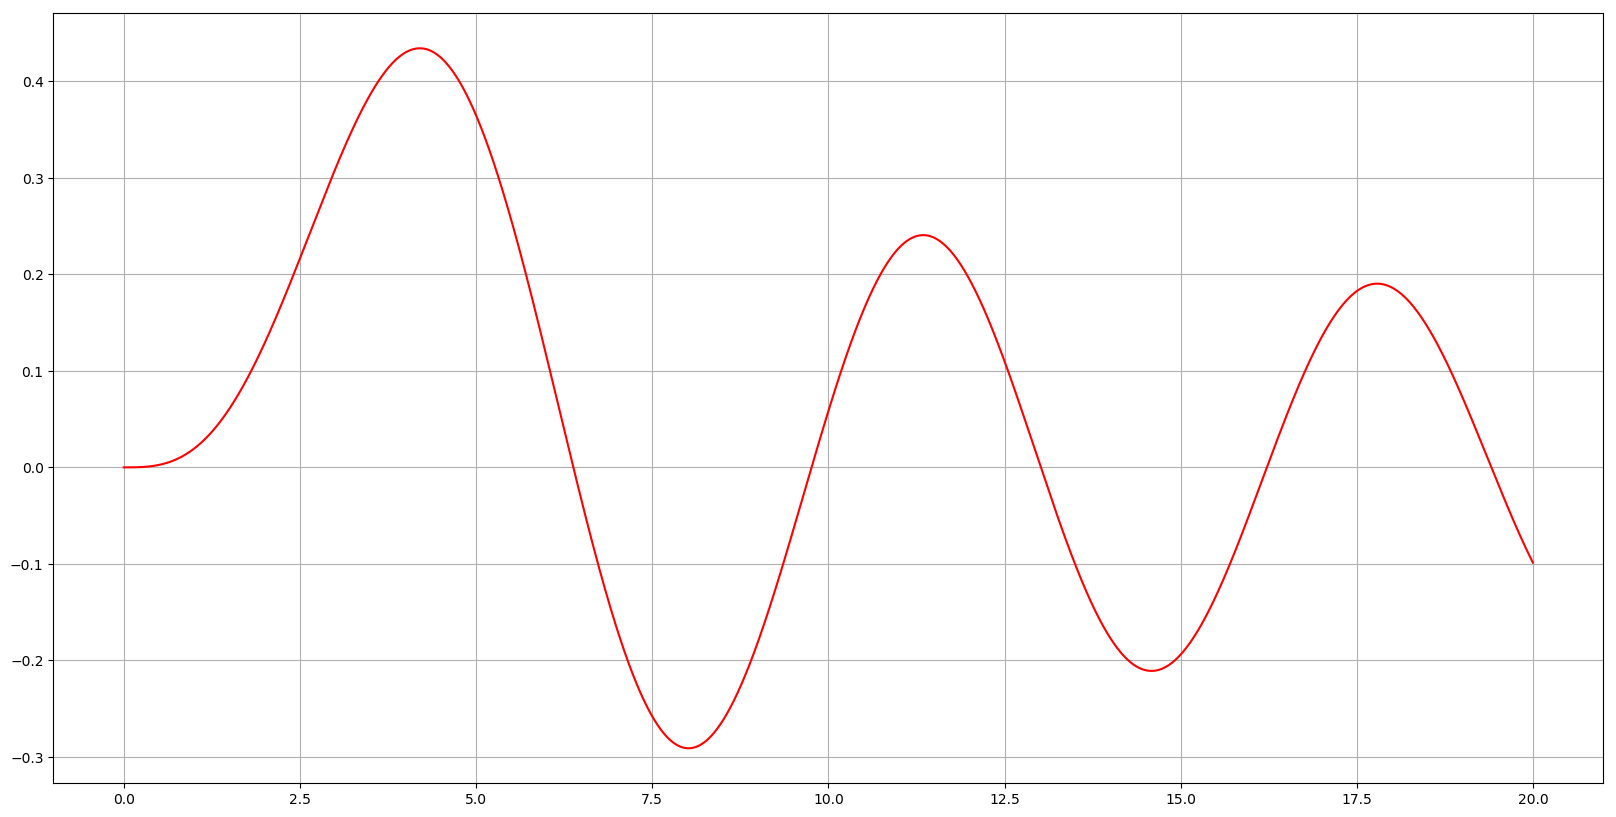
\includegraphics[width=\textwidth]{{../img/23-j3}.png}
	\caption{$J_3(x)$}
\end{figure}
\begin{figure}[H]
	\centering
	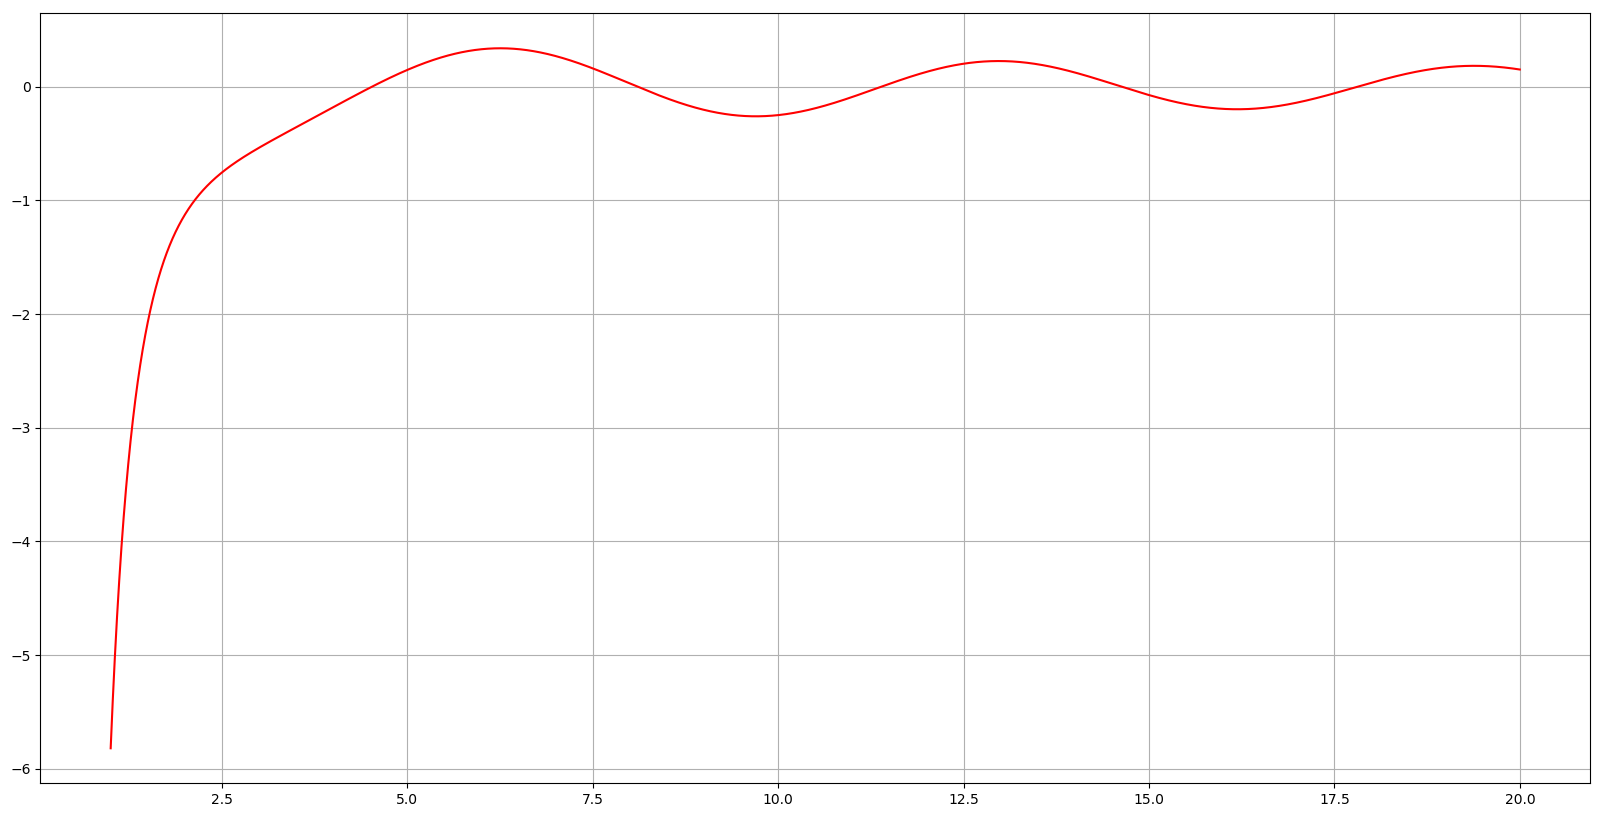
\includegraphics[width=\textwidth]{{../img/23-n3}.png}
	\caption{$N_3(x)$}
\end{figure}
 
Другий клас функцій Бесселя --- функції Бесселя уявного аргументу можна отримати як два лінійно–незалежних розв'язки рівняння \eqref{eq:4.7.2}, зокрема їх можна записати за формулою \eqref{eq:4.7.10} з використанням заміни змінної $x := i x$ в результаті будемо мати функцію Бесселя першого роду уявного аргументу:
\begin{equation}
	\label{eq:4.7.17}
	I_\nu(x) = \frac{J_\nu(i x)}{i^\nu} = \Sum_{k = 0}^\infty \frac{(x/2)^{2 k + \nu}}{k! \cdot \Gamma(k + \nu + 1)}, \quad 0 < x < \infty.
\end{equation}

Другий лінійно-незалежний розв'язок для нецілих $\nu$ можна отримати аналогічно попередньому розв'язку з формули \eqref{eq:4.7.10'}:
\begin{equation}
	\label{eq:4.7.18}
	I_{-\nu}(x) = i^\nu J_{-\nu}(i x) = \Sum_{k = 0}^\infty \frac{(x/2)^{2 k - \nu}}{k! \cdot \Gamma(k - \nu + 1)}, \quad 0 < x < \infty.
\end{equation}

Легко бачити, що при $\nu = n$ функції $I_n(x) = I_{-n}(x)$, тобто є лінійно залежними між собою і не можуть бути використані для запису загального розв'язку рівняння \eqref{eq:4.7.2}. \medskip

Функцію другого роду уявного аргументу будують у вигляді лінійної комбінації
\begin{equation}
	\label{eq:4.7.19}
	K_\nu(x) = \frac{\pi (I_{-\nu}(x) - I_\nu(x))}{2 \sin (\nu \pi)}.
\end{equation}

Враховуючи, що $I_n(x) = I_{-n}(x)$, остання формула має невизначеність типу $0/0$ при $\nu = n$. Розкриваючи її за правилом Лопіталя отримаємо 
\begin{equation}
	\label{eq:4.7.20}
	K_n(x) = \frac{(-1)^n}{2} \left( \left( \frac{\partial I_{-\nu}(x)}{\partial \nu} \right)_{\nu = n} - \left( \frac{\partial I_\nu(x)}{\partial \nu} \right)_{\nu = n} \right).
\end{equation}

\begin{definition}
	Функцію $K_\nu(x)$ називають функцією другого роду уявного аргументу, або функцією Макдональда вона має наступний вигляд:
	\begin{equation}
		\label{eq:4.7.21}
		\begin{aligned}
			K_n(x) &= -I_n(x) \ln \frac{x}{2} + \frac{1}{2} \Sum_{k = 0}^\infty \frac{(x/2)^{n + 2 k}}{k! (n - k)!} \left( \Psi(k + 1) + \Psi(k + n + 1) \right) + \\
			& \quad + \frac{1}{2} \Sum_{k=0}^{n-1} \frac{(-1)^k (n - k - 1)!}{k!} \left(\frac{2}{x}\right)^{n-2k}.
		\end{aligned}
	\end{equation}
\end{definition}

Виходячи з рекурентних співвідношень \eqref{eq:4.7.14}, \eqref{eq:4.7.14'}, можна отримати рекурентні співвідношення для функцій Бесселя уявного аргументу першого та другого роду:
\begin{gather}
	\label{eq:4.7.22}
	\frac{\diff}{\diff x} I_\nu(x) - \frac{\nu}{x} \cdot I_\nu(x) = I_{\nu+1}(x) \qquad \frac{\diff}{\diff x} I_\nu(x) + \frac{\nu}{x} \cdot I_\nu(x) = I_{\nu-1}(x), \\
	\label{eq:4.7.23}
	\frac{\diff}{\diff x} K_\nu(x) + \frac{\nu}{x} \cdot K_\nu(x) = -K_{\nu-1}(x) \qquad \frac{\diff}{\diff x} K_\nu(x) + \frac{\nu}{x} \cdot K_\nu(x) = -K_{\nu+1}(x).
\end{gather}

Відмітимо також характер поведінки функцій Бесселя уявного аргументу при $x = 0$ та $x \to \infty$. \medskip

Виходячи з формул \eqref{eq:4.7.17} та \eqref{eq:4.7.21} можна зробити висновок, що
\begin{gather}
	\label{eq:4.7.24}
	I_\nu(x) = O(x^\nu), \quad x \to 0, \\
	\label{eq:4.7.25}
	K_\nu(x) = O(x^{-\nu}), \quad \nu > 0, \qquad K_0(x) = O(\ln(x)), \quad x \to 0, \\
	\label{eq:4.7.26}
	I_\nu(x) \approx \sqrt{\frac{1}{2 \pi x}} \cdot e^x, \qquad K_\nu(x) \approx \sqrt{\frac{\pi}{2 x}} \cdot e^{-x}, \quad x \to \infty.
\end{gather}

Наведемо графіки функцій $I_3(x)$ та $K_3(x)$:
\begin{figure}[H]
	\centering
	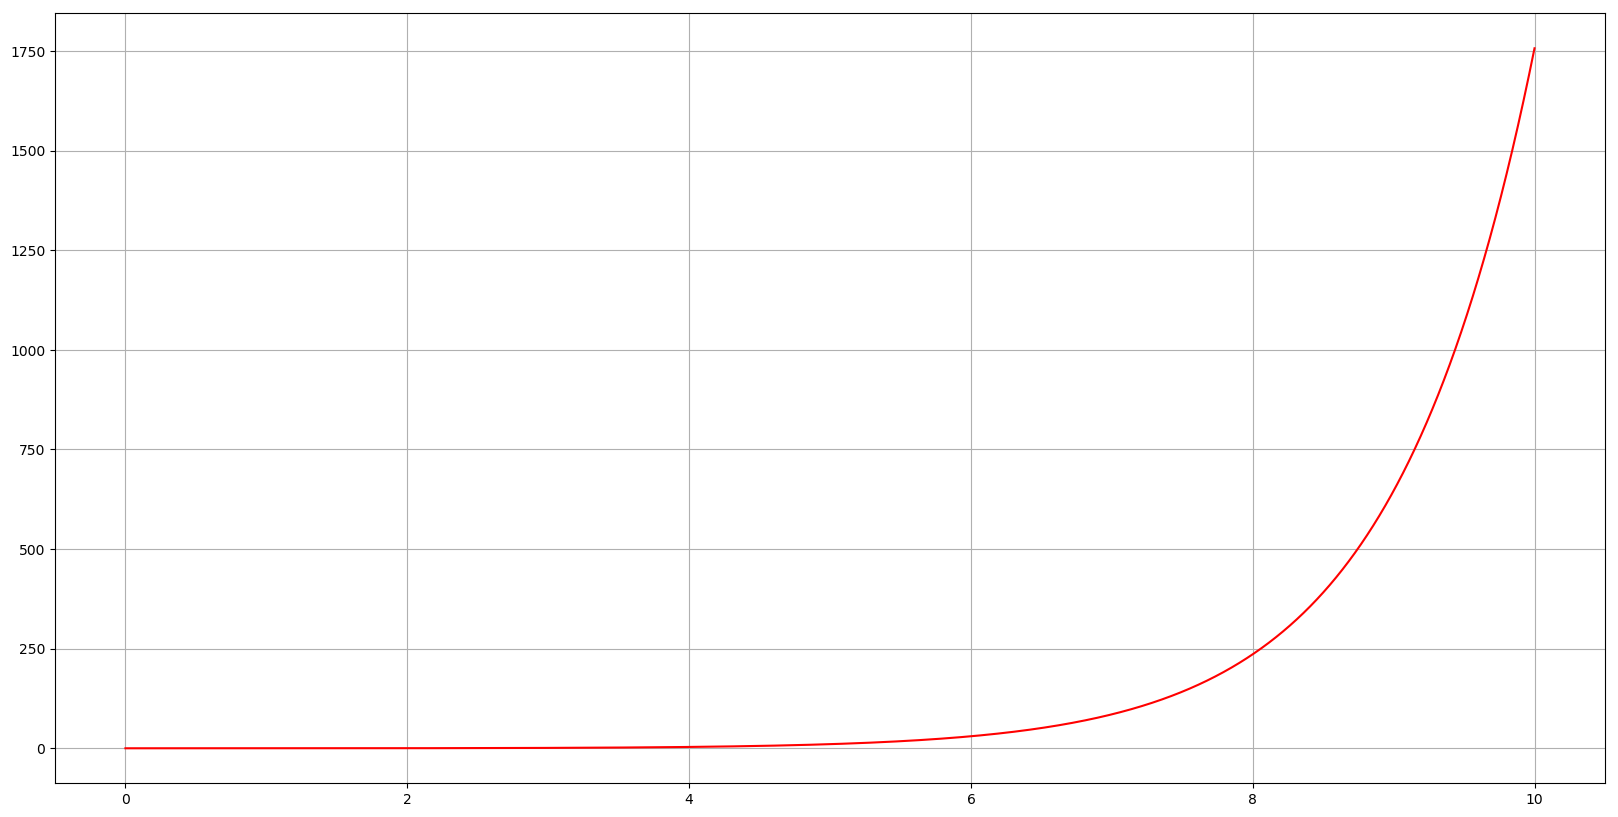
\includegraphics[width=\textwidth]{{../img/23-i3}.png}
	\caption{$I_3(x)$}
\end{figure}
\begin{figure}[H]
	\centering
	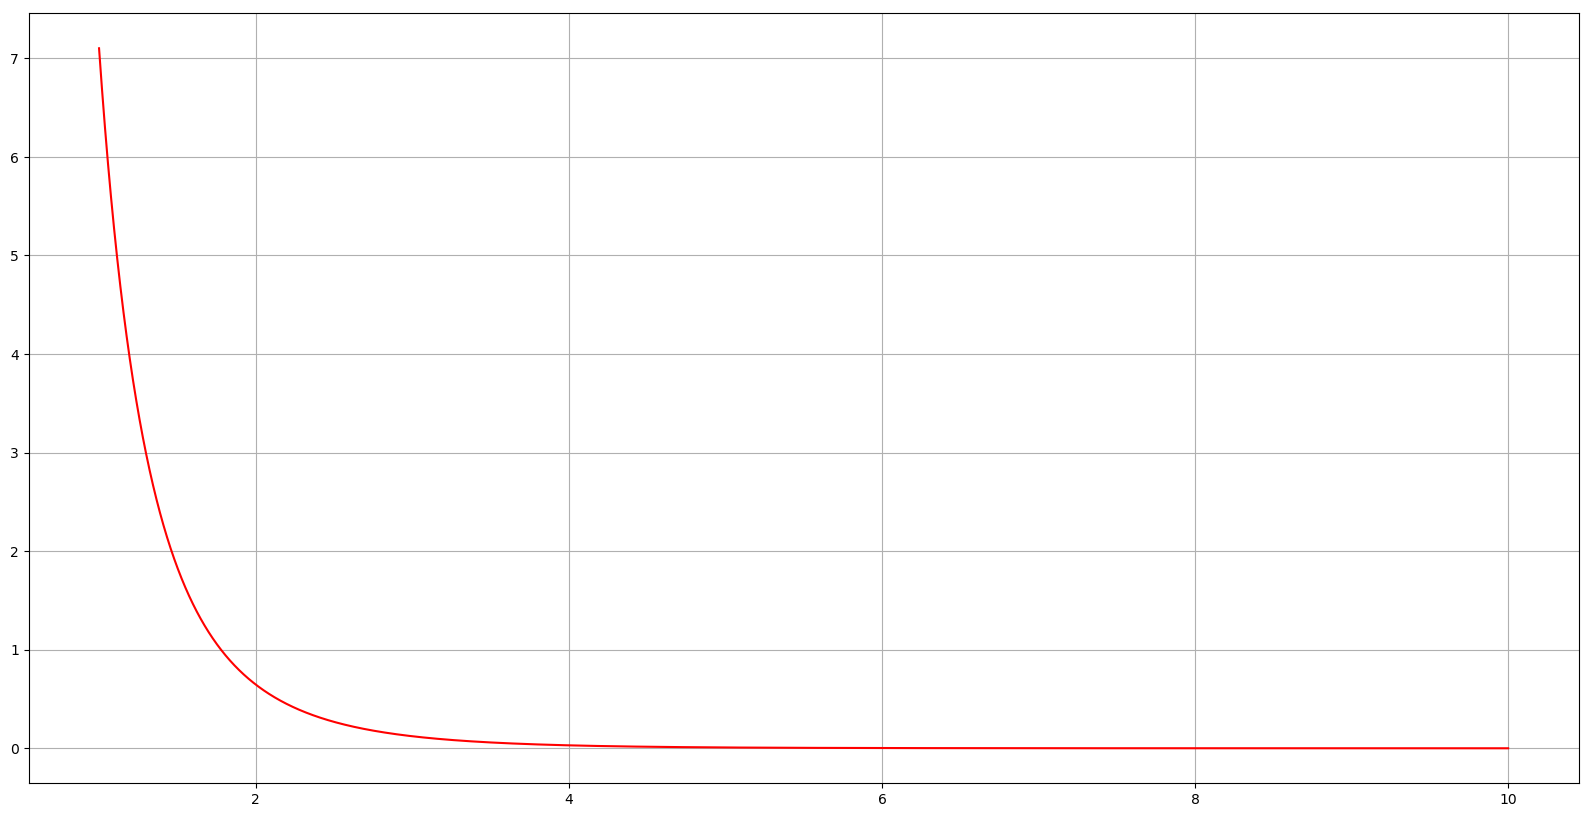
\includegraphics[width=\textwidth]{{../img/23-k3}.png}
	\caption{$K_3(x)$}
\end{figure}

\end{document}